\documentclass[11pt]{article}
\usepackage[margin=1in]{geometry}
\usepackage{amsmath,amssymb,amsthm,bm}
\usepackage{graphicx}
\usepackage{booktabs}
\usepackage[numbers]{natbib}
\usepackage[colorlinks=true,linkcolor=blue,citecolor=blue,urlcolor=blue]{hyperref}
\usepackage{microtype}
\usepackage{algorithm}
\usepackage{algpseudocode}
\usepackage{tikz}
\usetikzlibrary{positioning,arrows.meta,calc}

\newtheorem{theorem}{Theorem}
\newtheorem{assumption}{Assumption}
\newtheorem{proposition}{Proposition}
\newtheorem{corollary}{Corollary}
\theoremstyle{remark}
\newtheorem{remark}{Remark}
\newcommand{\E}{\mathbb{E}}
\newcommand{\Pn}{P_n}
\newcommand{\ind}{\mathbf{1}}

\title{Targeted Deep Survival Contrasts: Valid Inference for\\ Treatment-Specific Survival Benefit with Neural Networks}
\author{David McCoy$^{1}$ \quad Yi Li$^{1}$ \quad Mark J.\ van der Laan$^{1}$\\[4pt]
\small $^1$Division of Biostatistics, University of California, Berkeley}
\date{\small Draft --- \today}

\begin{document}
\maketitle

\begin{abstract}
Clinical deployment of neural survival models increasingly requires \emph{counterfactual} claims---how much a treatment would change survival in a population---not just prognostic risk scores. Such claims demand valid inference for treatment-specific survival contrasts under confounding and covariate-dependent censoring, targets for which standard deep survival estimators are biased and provide no honest uncertainty. Building on Targeted Deep Architectures (TDA), which embeds TMLE in a network's weight space, we target the full vector of treatment-specific survival curves $\{S_1(t), S_0(t)\}$ over a time grid, and hence the benefit curve $S_1(t)-S_0(t)$ and the restricted mean survival time (RMST) difference. A single universal targeting path---a ridge projection of the stacked efficient influence functions onto closed-form last-layer gradients---simultaneously solves the projected estimating equations for all coordinates within the neural working submodel, a one-step residual top-up restores the unrestricted target, and a multiplier bootstrap yields simultaneous confidence bands for the benefit curve over a prespecified time grid. In 200-replication simulations with confounded treatment, sign-varying effect heterogeneity, and censoring that depends on treatment and covariates, our estimator attains nominal pointwise coverage (95.6\%) and near-nominal simultaneous band coverage (94.0\%), with benefit-curve bias roughly a third of---and intervals 8\% narrower than---a per-timepoint one-step (AIPCW) correction built from the same nuisance fits at comparable coverage; a head-to-head mechanism study shows both of TDSC's ingredients matter, with MSE improving from one-step to output-space survival TMLE to TDSC on identical nuisances, an isotonized one-step closing essentially none of the gap, and causal survival forests carrying visible regularization bias into this population-level target. We provide formal guarantees---joint asymptotic linearity across all coordinates, simultaneous-band validity, and a residual ``top-up'' that provably restores double robustness---for a cross-fitted variant requiring no Donsker conditions, which is empirically nominal at a quantified efficiency cost (about a third wider intervals). Misspecification and small-sample experiments delineate a three-tier operating envelope: weight-space targeting delivers the best finite-sample efficiency in the well-specified scenarios considered and is the most exposed when the initial fit fails, with the output-space TMLE intermediate and the one-step the reliable fallback.
\end{abstract}

\section{Introduction}\label{sec:intro}

Neural networks are now standard tools for individual-level survival prediction from rich clinical inputs, including digital pathology and other high-dimensional modalities. Clinical decisions, however, hinge on \emph{contrasts}: how survival would differ under one treatment versus another. Estimating such contrasts from observational data raises two familiar obstacles---confounding and censoring that depends on treatment and covariates---and a less appreciated third: a network trained for predictive loss is a biased, inefficient estimator of any low-dimensional causal functional \citep{chernozhukov2018dml,shi2019dragonnet}, and its naive standard errors are invalid.

Semiparametric theory offers the remedy: debias a flexible initial fit by solving the efficient influence function (EIF) equation, via one-step/AIPCW corrections \citep{chernozhukov2018dml,kennedy2024review} or targeted maximum likelihood estimation (TMLE) \citep{vdl2011tl}. For survival targets these tools are mature \citep{moore2009,cai2020,rytgaard2024}, but standard implementations correct \emph{outside} the model: the one-step adds the empirical mean of the EIF to a plug-in, and classical TMLE fluctuates the output distribution after training. Both become awkward when the target is a whole \emph{vector}---two survival curves on a fine grid---where per-coordinate corrections need not respect monotonicity and can push estimates off the model space. Targeted Deep Architectures (TDA) \citep{li2025tda} instead embeds the TMLE fluctuation \emph{inside} the network: a small targeting subset of weights is updated along the projection of the EIF onto per-sample loss gradients, so the fitted network itself is the debiased estimator. TDA was demonstrated for the average treatment effect and the marginal survival curve without treatment; the clinically decisive object---the causal contrast of treatment-specific survival curves under confounding and dependent censoring---was not addressed.

\paragraph{Related work.} Neural estimators of treatment-specific survival curves exist---notably SurvITE \citep{curth2021survite}, which targets exactly our estimand with balanced discrete-time hazard networks, and counterfactual time-to-event models \citep{chapfuwa2021}---but they provide point estimates without valid confidence statements; that is the gap we fill. Conversely, survival TMLEs with simultaneous inference exist \citep{cai2020,rytgaard2024}, including universal one-dimensional least-favorable submodels that target an entire survival curve at once; but those universal paths are constructed \emph{analytically}, per estimand and likelihood. TDSC's contribution on this axis is not that a universal path exists---it is that the path is obtained \emph{generically} from the architecture's score gradients, with no estimand-specific analytic derivation, for any network and any stack of pathwise-differentiable targets. Causal survival forests \citep{cui2023csf} give honest inference for conditional effects at fixed horizons rather than the full population benefit curve.

\paragraph{Contributions.} We propose \emph{Targeted Deep Survival Contrasts} (TDSC): (1) the target vector $\Psi = (S_1(t_1),\dots,S_1(t_K), S_0(t_1),\dots,S_0(t_K))$ with its stacked EIFs combining treatment and censoring weights (Section~\ref{sec:setup}); (2) closed-form per-sample last-layer gradients making the universal targeting update for all $2K$ coordinates one ridge regression per iteration (Algorithm~\ref{alg:tdsc}), with multiplier-bootstrap sup-$t$ bands for the benefit curve (Section~\ref{sec:method}); (3) formal guarantees---joint asymptotic linearity, band validity, and a residual top-up that provably restores point-estimate double robustness---for a cross-fitted variant satisfying the sample-splitting premise of the underlying ADML theory, together with a design rule (and documented failure mode) for where the high-dimensional targeting step may be solved (Sections~\ref{sec:method}--\ref{sec:theory}); (4) a comprehensive simulation program---a 200-replication main study, nuisance-misspecification and sample-size grids, a cross-fitting comparison, and head-to-head external comparators (output-space survival TMLE, causal survival forests)---that decomposes the mechanism behind TDSC's gains and maps its operating envelope (Section~\ref{sec:sims}).

\section{Setup, estimands, and efficient influence functions}\label{sec:setup}

\paragraph{Data.} We observe $n$ i.i.d.\ copies of $O=(X, A, \tilde T, \Delta)$: covariates $X\in\mathbb{R}^d$, binary treatment $A\in\{0,1\}$, discrete follow-up time $\tilde T\in\{1,\dots,K\}$, event indicator $\Delta$. Time is coarsened into $K$ bins; within a bin, events are recorded before censoring, and subjects surviving bin $K$ are administratively censored. Let $Y(k)=\ind\{\tilde T\ge k\}$ (at risk) and $dN(k)=\ind\{\tilde T=k,\Delta=1\}$ (event), and write $\Pn f = n^{-1}\sum_i f(O_i)$. The likelihood factorizes through the propensity $g(X)=P(A=1\mid X)$, the event hazard $h(k\mid a,x)$, and the censoring hazard $h_c(k\mid a,x)$, with conditional survival $S(t\mid a,x)=\prod_{k\le t}\{1-h(k\mid a,x)\}$ and censoring survival $S_c$ defined analogously.

\paragraph{Estimands.} Under consistency, no unmeasured confounding, coarsening-at-random censoring (censoring may depend on $A$ and $X$ but not further on the event time), and positivity for treatment and censoring, the treatment-specific curves
$S_a(t) = \E_X[S(t \mid a, X)]$, $a\in\{0,1\}$, $t\in\{1,\dots,K\}$,
are identified. Our target is the $2K$-vector $\Psi=(S_1(\cdot), S_0(\cdot))$; the \emph{benefit curve} $\beta(t)=S_1(t)-S_0(t)$ and the RMST difference $\Delta_{\mathrm{RMST}}=\sum_{t=1}^{K}\beta(t)$ (bin width one; the contrast in expected bins survived through horizon $K$) are linear in $\Psi$, so their influence functions follow by linearity.

\paragraph{Efficient influence functions.} For each coordinate $S_a(t)$ the EIF at $P$ is the discrete-time analogue of \citet{moore2009}:
\begin{equation}\label{eq:eif}
D_{a,t}(O) \;=\; -\sum_{k=1}^{t} \frac{\ind\{A=a\}}{g_a(X)\, S_c(k-1\mid a, X)}\,\frac{S(t\mid a,X)}{S(k\mid a,X)}\Big(dN(k) - Y(k)\, h(k\mid a,X)\Big) \;+\; S(t\mid a,X) - S_a(t),
\end{equation}
with $g_1=g$, $g_0=1-g$. The first term is a weighted sum of martingale residuals---the within-bin ``surprise'' of an event relative to the fitted hazard---inversely weighted by the probability of receiving arm $a$ and remaining uncensored through bin $k-1$; the second is the plug-in centering term. Stacking \eqref{eq:eif} over $a$ and $t$ gives the $n\times 2K$ influence matrix $D$ whose column means $\Pn D_{a,t}$ are the first-order bias terms; the restricted targeting step drives their \emph{projections} onto the working score span to zero, and the residual top-up removes what remains.

\section{Targeted Deep Survival Contrasts}\label{sec:method}

\paragraph{Architecture and initial fit.} We use a DragonNet-style network \citep{shi2019dragonnet} adapted to discrete-time survival: a shared trunk feeding a propensity head for $g$ and two outcome heads producing hazard logits $\{h(k\mid a, x)\}_{k=1}^{K}$ for $a\in\{0,1\}$, trained on the observed-arm discrete-time negative log-likelihood (masked per-bin binary cross-entropy) plus a propensity term, with early stopping. A separate network fits the censoring hazard. Any backbone---including a frozen foundation-model encoder with a trained head---can replace the trunk. Full architecture and hyperparameters are in Appendix~\ref{app:repro}.

\begin{figure}[t]
\centering
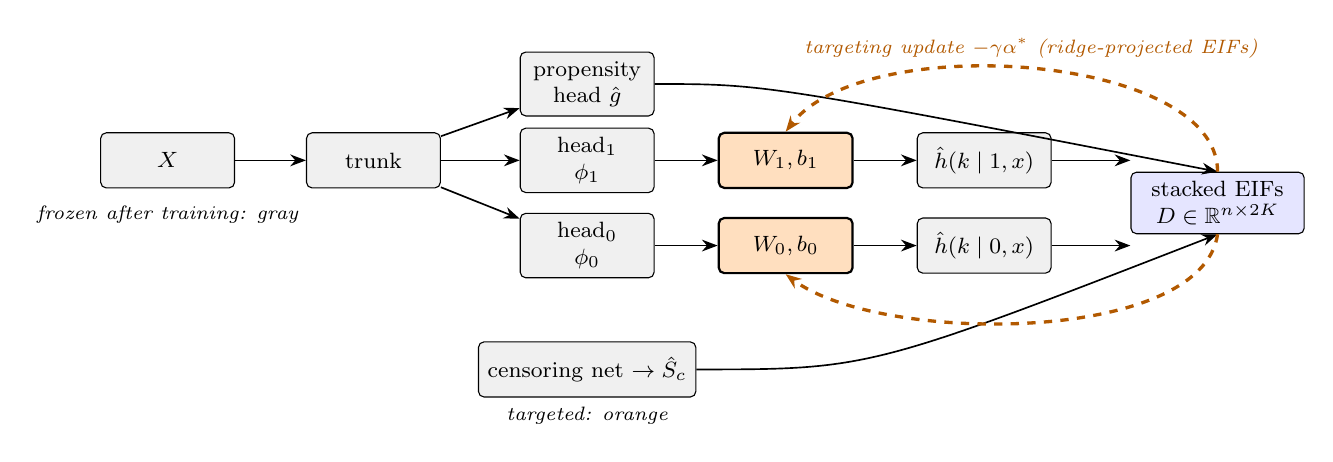
\begin{tikzpicture}[
  box/.style={draw, rounded corners=2pt, minimum height=7mm, minimum width=17mm, font=\footnotesize, align=center},
  frozen/.style={box, fill=gray!12},
  targ/.style={box, fill=orange!25, thick},
  lab/.style={font=\scriptsize\itshape},
  arr/.style={-{Stealth[length=2mm]}, semithick}]
\node[frozen] (X) {$X$};
\node[frozen, right=9mm of X] (trunk) {trunk};
\node[frozen, above right=2mm and 10mm of trunk] (g) {propensity\\head $\hat g$};
\node[frozen, right=10mm of trunk] (phi1) {head$_1$\\$\phi_1$};
\node[frozen, below=2.5mm of phi1] (phi0) {head$_0$\\$\phi_0$};
\node[targ, right=8mm of phi1] (W1) {$W_1, b_1$};
\node[targ, right=8mm of phi0] (W0) {$W_0, b_0$};
\node[frozen, right=8mm of W1] (h1) {$\hat h(k\mid 1,x)$};
\node[frozen, right=8mm of W0] (h0) {$\hat h(k\mid 0,x)$};
\node[frozen, below=8mm of phi0] (cens) {censoring net $\to \hat S_c$};
\node[box, fill=blue!10, right=10mm of $(h1.east)!0.5!(h0.east)$, minimum width=22mm] (eif) {stacked EIFs\\$D \in \mathbb{R}^{n\times 2K}$};
\draw[arr] (X) -- (trunk);
\draw[arr] (trunk) -- (g);
\draw[arr] (trunk) -- (phi1);
\draw[arr] (trunk) -- (phi0);
\draw[arr] (phi1) -- (W1);
\draw[arr] (phi0) -- (W0);
\draw[arr] (W1) -- (h1);
\draw[arr] (W0) -- (h0);
\draw[arr] (h1.east) -- (eif.west|-h1.east);
\draw[arr] (h0.east) -- (eif.west|-h0.east);
\draw[arr] (g.east) .. controls +(14mm,0mm) .. (eif.north);
\draw[arr] (cens.east) .. controls +(22mm,0mm) .. (eif.south);
\draw[arr, dashed, orange!70!black, very thick]
  (eif.north) .. controls +(0,15mm) and +(10mm,13mm) .. node[above, lab, text=orange!70!black]{targeting update $-\gamma\alpha^\ast$ (ridge-projected EIFs)} (W1.north);
\draw[arr, dashed, orange!70!black, very thick]
  (eif.south) .. controls +(-2mm,-14mm) and +(12mm,-9mm) .. (W0.south);
\node[lab, below=1mm of X] {frozen after training: gray};
\node[lab, below=0mm of cens, xshift=0mm] {targeted: orange};
\end{tikzpicture}
\caption{TDSC pipeline. A DragonNet-style survival network produces per-arm hazards; the propensity head and a separate censoring network supply the weights inside the stacked EIFs. Only the final linear layers $(W_a, b_a)$ are updated, along the universal direction obtained by ridge-projecting all $2K$ EIFs onto their closed-form per-sample gradients; everything else stays frozen.}
\label{fig:pipeline}
\end{figure}

\paragraph{Targeting submodel and closed-form gradients.} Following TDA, the targeting parameters $\vartheta$ are the final linear layers of the two outcome heads, $p = 2K(F{+}1)$ parameters for head width $F$. Because those layers are linear in the head features $\phi_a(X)$ and the loss is a per-bin Bernoulli likelihood, the per-sample gradient is available in closed form:
\begin{equation}\label{eq:grad}
\frac{\partial \ell_i}{\partial W_a[k,\cdot]} = \ind\{A_i=a\}\, Y_i(k)\big(h(k\mid a, X_i) - dN_i(k)\big)\, \phi_a(X_i),
\end{equation}
and analogously for biases, giving the $n\times p$ score matrix $G$ in one vectorized pass with no per-sample automatic differentiation.

\begin{figure}[t]
\centering
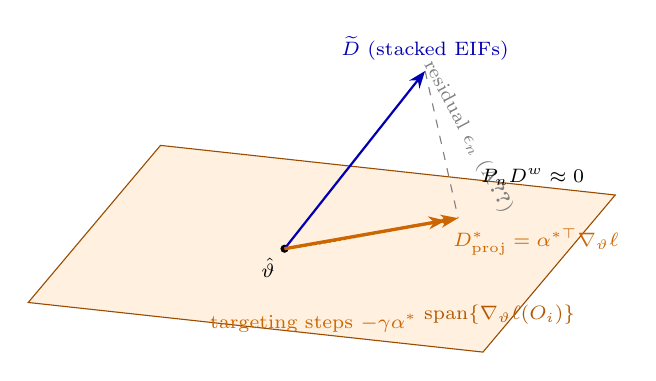
\begin{tikzpicture}[scale=1.05, arr/.style={-{Stealth[length=2.2mm]}, thick}, lab/.style={font=\scriptsize}]
% score span (plane)
\draw[fill=orange!12, draw=orange!60!black]
  (-3.1,-0.9) -- (2.4,-1.5) -- (4.0,0.4) -- (-1.5,1.0) -- cycle;
\node[lab, orange!70!black] at (2.6,-1.05) {$\mathrm{span}\{\nabla_{\vartheta}\ell(O_i)\}$};
% origin
\coordinate (O) at (0,-0.25);
\fill (O) circle (1.4pt);
\node[lab, below left=0mm of O] {$\hat\vartheta$};
% EIF vector off-plane
\coordinate (D) at (1.7,1.9);
\draw[arr, blue!70!black] (O) -- (D) node[above, lab, text=blue!70!black] {$\widetilde D$ (stacked EIFs)};
% projection in-plane
\coordinate (P) at (2.1,0.12);
\draw[arr, orange!80!black, very thick] (O) -- (P) node[below right=0mm and -2mm, lab, text=orange!80!black] {$D^{\ast}_{\mathrm{proj}} = \alpha^{\ast\top}\nabla_{\vartheta}\ell$};
% residual
\draw[dashed, gray] (D) -- (P);
\node[lab, gray, rotate=-62] at (2.22,1.1) {residual $\epsilon_n$ (A\ref{a:span})};
% iterative path along plane
\draw[arr, orange!80!black, densely dotted, semithick]
  (O) .. controls (0.8,-0.15) and (1.4,0.02) .. (1.95,0.09);
\node[lab, orange!80!black] at (0.35,-1.15) {targeting steps $-\gamma\alpha^{\ast}$};
% target set
\fill[orange!80!black] (1.95,0.09) circle (1.3pt);
\node[lab] at (3.0,0.62) {$\Pn D^{w} \approx 0$};
\end{tikzpicture}
\caption{Geometry of the targeting update. The stacked nonparametric EIFs $\widetilde D$ are projected onto the span of the per-sample loss gradients of the targeting parameters; TDSC steps $\vartheta$ along the projected direction until the \emph{projected} estimating equations hold. The observable residual $\epsilon_n$ (Assumption~\ref{a:span}) measures how much of the nonparametric EIF lies outside the working score span---the gap between the two influence-function geometries and the potential efficiency gain from the restriction, not the parameter-value bias, which the oracle-bias conditions govern separately---and the full-EIF means it leaves behind are exactly what the one-step residual top-up adds back.}
\label{fig:geometry}
\end{figure}

\paragraph{Universal targeting update.} Each iteration solves one ridge system for all $2K$ targets, $\alpha = (G^\top G + \lambda I)^{-1} G^\top D$ (with $\lambda$ scaled to the mean diagonal of $G^\top G$; note $p>n$ here, so the ridge penalty is statistically active), giving per-target directions $\alpha_j$ and projected bias terms $d_j = \Pn[G\alpha_j]$. Writing $D^{w} = G\alpha$ for the resulting \emph{working-submodel} influence functions, the universal direction is $\alpha^* = \sum_j (d_j/\|d\|_2)\, \alpha_j$ \citep[Sec.~2.3]{li2025tda}, applied as $\vartheta \leftarrow \vartheta - \gamma\,\alpha^*$ with a backtracking line search on $\sum_j(\Pn D^{w}_j)^2$ ($\alpha$ held fixed within the search). After each accepted step the hazards, influence matrix, and projection are recomputed ($g$ and $S_c$ stay fixed). \emph{The stopping criterion is the projected one}: iteration ends when every $|\Pn D^{w}_j| \le \widehat{\mathrm{sd}}(D^{w}_j)/(\sqrt{n}\log n)$---the estimating equations of the working submodel, which the restricted parameterization can actually solve. The \emph{full}-EIF means $\Pn D_j$ need not vanish inside a restricted submodel; they are tracked as a diagnostic, and adding them back as a one-step residual top-up, $\widehat\Psi + \Pn D$, converts the plug-in into an estimator of the unrestricted target (Proposition~\ref{prop:dr}). The second diagnostic is the relative projection residual $\|D - D^{w}\|/\|D\|$, whose interpretation Section~\ref{sec:theory} makes precise: it measures how much of the nonparametric EIF lies outside the working score span---the gap between the two influence-function \emph{geometries}, hence the potential efficiency gain from the restriction---not the parameter-value bias $\Psi_n(P_0) - \Psi(P_0)$, which is governed separately by the oracle-bias conditions. The plug-in estimator is, by construction, a pair of monotone survival curves.

\begin{algorithm}[t]
\caption{TDSC universal targeting (no-split form)}
\label{alg:tdsc}
\begin{algorithmic}[1]
\Require trained hazard/propensity network and censoring network; targeting parameters $\vartheta$ (final layers of the outcome heads); ridge scale $\lambda$
\State fix weights $\hat g, \hat S_c$; compute hazards $\hat h_a$, survival curves, and stacked full EIFs $D\in\mathbb{R}^{n\times2K}$ via \eqref{eq:eif}
\Loop
    \State $G \gets$ per-sample loss gradients w.r.t.\ $\vartheta$ \Comment{closed form \eqref{eq:grad}; no autograd}
    \State $\alpha \gets (G^\top G + \lambda I)^{-1} G^\top D$; \quad $D^{w} \gets G\alpha$ \Comment{working-submodel EIFs}
    \State \textbf{if} $|\Pn D^{w}_j| \le \widehat{\mathrm{sd}}(D^{w}_j)/(\sqrt n\log n)$ for all $j$ \textbf{then break} \Comment{projected criterion}
    \State $d_j \gets \Pn D^{w}_j$; \quad $\alpha^\ast \gets \sum_j (d_j / \lVert d\rVert_2)\, \alpha_j$ \Comment{universal direction}
    \State backtracking line search: $\vartheta \gets \vartheta - \gamma\,\alpha^\ast$, accepting only if $\sum_j (\Pn D^{w}_j)^2$ falls ($\alpha$ fixed within the search); \textbf{break} if no $\gamma$ improves
    \State recompute $\hat h_a$, curves, and $D$ at the updated $\vartheta$
\EndLoop
\State \Return plug-ins $\widehat\Psi_j$; full-residual top-up $\widehat\Psi_j + \Pn D_j$; plug-in SEs $\widehat{\mathrm{sd}}(D^{w}_j)/\sqrt n$, top-up SEs $\widehat{\mathrm{sd}}(D_j)/\sqrt n$; multiplier-bootstrap band; diagnostics ($\lVert D - D^{w}\rVert/\lVert D\rVert$, $\max_j|\Pn D_j|$)
\end{algorithmic}
\end{algorithm}

\paragraph{Cross-fitted variant.} To satisfy the sample-splitting premise of the theory below without Donsker conditions on the network class, TDSC admits a $V$-fold cross-fitted form: for each fold, the nuisance networks are trained \emph{and targeted} on the complement; the held-out fold then supplies evaluation---plug-in curves, influence functions at the targeted fit, and an exact residual correction $P_{n,v}[D]$ so the EIF equations hold exactly on held-out data (by Proposition~\ref{prop:dr}, a cross-fitted one-step at the targeted nuisances). Fold contributions are averaged; the pooled per-observation influence matrix supplies variance and bands.

\paragraph{Why not target fold-wise on the held-out folds?} A tempting alternative solves the EIF equations with the full targeting submodel \emph{separately on each held-out fold}. This fold-wise high-dimensional targeting fails badly here, and the mechanism is instructive. It is \emph{not} what classical CV-TMLE \citep{zheng2011cvtmle} does: there, a single \emph{low-dimensional} fluctuation is fit by pooling the cross-validated loss over all validation folds---$O(1)$ parameters against $n$ observations---which is exactly why it is safe (the faithful CV-TMLE analogue here would pool the $2K$ one-dimensional fluctuations of Section~\ref{sec:sims}'s output-space TMLE across folds, which we have not run). TDA's submodel, by contrast, is the network's final layers ($p \approx 4{,}000$ here), so on a fold of $n/V\approx200$ observations the gradient matrix has rank at most $200$ and the fold's empirical EIF equations can be solved nearly exactly---by fitting the fold's \emph{sampling noise}, whose order $\mathrm{sd}(D)/\sqrt{n/V}$ rivals the genuine first-order bias the step is meant to remove. The resulting hazard perturbations pass through the nonlinear map $h \mapsto \prod_k(1-h(k))$, rectifying symmetric fold-level fluctuation into systematic bias, and the fold-fitted targeting layers reintroduce exactly the empirical-process term $(\Pn - P_0)(\widehat D - D_0)$ that cross-fitting is meant to eliminate---now concentrated on the smallest split. Empirically this variant gave 14-fold larger benefit-curve bias than the no-split estimator, 70.5\% pointwise and 42\% simultaneous coverage (100 replications; store preserved in the repository). The design rule: the dimension of the data-adaptive targeting step must be small relative to the split on which its equations are solved, so targeting belongs with training on the large split, and the held-out fold should receive only evaluation and the linear residual correction. Section~\ref{sec:sims} compares the no-split and cross-fitted forms empirically.

\paragraph{Inference and simultaneous bands.} Two variance prescriptions correspond to the two inferential targets of Section~\ref{sec:theory}: the \emph{top-up} estimator (unrestricted target) uses the full-EIF standard errors $\widehat{\mathrm{sd}}(D_j)/\sqrt n$, while the \emph{plug-in} (working target) uses the working-submodel standard errors $\widehat{\mathrm{sd}}(D^{w}_j)/\sqrt n$, both at the final fit; contrasts inherit influence functions by linearity. For the benefit curve we report a sup-$t$ band over the prespecified grid: with i.i.d.\ standard normal multipliers $\xi_i$ and centered influence values $\bar D_{\beta,t} = \Pn D_{\beta,t}$, the 95\% quantile $c^*$ of $\max_t |n^{-1}\sum_i \xi_i \{D_{\beta,t}(O_i) - \bar D_{\beta,t}\}|/\widehat{\mathrm{se}}_t$ over bootstrap draws gives $\hat\beta(t) \pm c^*\widehat{\mathrm{se}}_t$ ($c^*$ floored at 1.96, a conservative choice).

\section{Theory}\label{sec:theory}

TDSC is TDA applied to a $2K$-dimensional pathwise-differentiable target, and its guarantees specialize those of \citet[Thms.~3.1--3.2]{li2025tda} and adaptive debiased machine learning (ADML) \citep{vdl2023adml}. We state the specialization for the \emph{cross-fitted} implementation (Section~\ref{sec:method}; $V$-fold, nuisances trained and targeted out-of-fold, evaluation with exact residual correction on the held-out fold), which satisfies the sample-splitting premise of those results without Donsker conditions on the network class.

Three influence-function objects must be kept distinct. $D^{\mathrm{np}}_0$ denotes the $2K$-vector of \emph{nonparametric} EIFs \eqref{eq:eif} at $P_0$---the influence function of the unrestricted target $\Psi(P_0)$. $M_n\subseteq\mathcal M$ is the data-adaptive working submodel induced by partially unfreezing $\vartheta$, with working parameter $\Psi_n(P_0)=\Psi(\Pi_n P_0)$ and \emph{working-model} EIF $D^{w}_n$, the (unpenalized) $L^2(P_0)$-projection of $D^{\mathrm{np}}_0$ onto the closure of the working score span. What the algorithm computes is the ridge-regularized empirical counterpart, $\widehat D^{w,\lambda} = G\widehat\alpha_\lambda$ with $\widehat\alpha_\lambda = (G^\top G + \lambda I)^{-1}G^\top D$; wherever $\widehat D^{w,\lambda}$ stands in for $D^{w}_n$ (the stopping rule, the plug-in standard errors) we assume $\|\widehat D^{w,\lambda} - D^{w}_n\|_{P_0} = o_p(1)$, for which it suffices that the \emph{relative} ridge vanish, $\lambda_n / \mathrm{mean\,diag}(G^\top G) \to 0$; our simulations fix that ratio at $0.01$ as a finite-sample stabilizer, and its sensitivity is examined in Section~\ref{sec:sims}. Under ADML there is additionally an oracle submodel with EIF $D^{O}$ to which $D^{w}_n$ converges; the estimators below are asymptotically linear with $D^{\mathrm{np}}_0$ (top-up) or $D^{O}$ (plug-in), and conflating the two is what a careless reading invites---the entire variance story lives in the gap between them.

\begin{assumption}[Identification and positivity]\label{a:id}
Consistency, no unmeasured confounding, coarsening-at-random censoring; and $\delta \le g_0(X) \le 1-\delta$, $S_{c,0}(K-1\mid a, X)\ge\delta$ a.s.\ for some $\delta>0$.
\end{assumption}
\begin{assumption}[Nuisance rates]\label{a:rates}
For $f = f(k, a, x)$ write $\|f\|_{P_0}^2 = \sum_{a}\sum_{k=1}^{K} \E_{P_0} f(k,a,X)^2$. The cross-fitted weight estimators and the \emph{targeted} per-fold hazard estimators are each consistent in $\|\cdot\|_{P_0}$, respect the bounds of Assumption~\ref{a:id}, and satisfy the product rate $\|\hat h - h_0\|_{P_0}\big(\|\hat g - g_0\|_{P_0} + \|\hat S_c - S_{c,0}\|_{P_0}\big) = o_p(n^{-1/2})$ (a sufficient condition for the sharper per-$(a,t)$ sums of per-bin products appearing in the remainder).
\end{assumption}
\begin{assumption}[Gradient coverage---plug-in story only]\label{a:span}
The projection residual $\epsilon_{n,j} = D^{\mathrm{np}}_{0,j} - D^{w}_{n,j}$ stabilizes: $D^{w}_n$ converges in $L^2(P_0)$ to an oracle-model EIF $D^{O}$. \emph{This assumption is not required for Theorem~\ref{thm:main}.} It governs only the plug-in story (Proposition~\ref{prop:plugin}), and the size of $\|\epsilon_n\|$ is a dial, not a defect---but note carefully what it measures: the residual is a statement about influence-function \emph{geometry}, not parameter values. Even when the oracle submodel contains $P_0$ (so $\Psi(\Pi_0 P_0) = \Psi(P_0)$ exactly and there is no approximation bias), $D^{O}$ can remain a strict projection of $D^{\mathrm{np}}_0$ onto a smaller tangent space, with $\mathrm{Var}(D^{O}) < \mathrm{Var}(D^{\mathrm{np}}_0)$---the same parameter with a lower local efficiency bound. That is the ADML superefficiency mechanism. Approximation bias $\Psi_n(P_0) - \Psi(P_0)$ is governed separately by the oracle-bias conditions (C1)--(C2). The empirical residual $\|D - \widehat D^{w,\lambda}\|/\|D\|$ estimates the geometric gap.
\end{assumption}

\begin{theorem}[Joint asymptotic linearity and efficiency of the top-up estimator]\label{thm:main}
The full-residual top-up estimator \emph{is} the cross-fitted AIPCW one-step evaluated at the targeted nuisances (Proposition~\ref{prop:dr}); no separate ``EIF equations solved'' condition is needed. Under Assumptions~\ref{a:id} and~\ref{a:rates} alone (Assumption~\ref{a:span} not required), $\widehat\Psi^{+}$ satisfies jointly in $\mathbb{R}^{2K}$
$\widehat\Psi^{+} - \Psi(P_0) = \Pn D^{\mathrm{np}}_{0} + o_p(n^{-1/2})$, so $\sqrt n\,(\widehat\Psi^{+} - \Psi(P_0)) \rightsquigarrow N(0, \Sigma_0)$ with $\Sigma_0 = P_0 D^{\mathrm{np}}_0 (D^{\mathrm{np}}_0)^\top$: the estimator is regular and attains the nonparametric efficiency bound. Targeting enters only through Assumption~\ref{a:rates}---it must not degrade, and is designed to improve, the targeted hazards' rates---so the theorem claims no asymptotic variance advantage for weight-space targeting; any benefit is finite-sample, through better nuisances.
\end{theorem}

\begin{proposition}[Cross-fitted plug-in: working parameter and superefficiency]\label{prop:plugin}
The cross-fitted TDSC \emph{plug-in} (no top-up) is instead an ADML-type estimator of the working parameter $\Psi_n(P_0) = \Psi(\Pi_n P_0)$: under Assumption~\ref{a:span} and the conditions of \citet[Thms.~3.1--3.2]{li2025tda}---including the oracle-bias conditions (C1)--(C2) under which $\Psi_n(P_0)$ may replace $\Psi(P_0)$---it is asymptotically linear with the oracle EIF $D^{O}$, whose variance is no larger than $\Sigma_0$ and strictly smaller whenever the projection residual of Assumption~\ref{a:span} does not vanish (superefficiency, with the usual ADML price: nonregularity for the unrestricted target under local alternatives outside the oracle model). Its inference must therefore use the \emph{working-model} standard errors $\widehat{\mathrm{sd}}(D^{w}_j)/\sqrt n$; pairing the plug-in with full-EIF standard errors is conservative. Both signatures---lower MSE than Theorem~\ref{thm:main}'s estimator, and over-coverage under full-EIF variance---appear in Section~\ref{sec:sims}.
\end{proposition}

\begin{corollary}[Contrasts]\label{cor:contrasts}
The benefit curve $\hat\beta(\cdot)$ and $\widehat\Delta_{\mathrm{RMST}}$ are asymptotically linear by linearity of both maps, with influence functions $D^{\mathrm{np}}_{\beta,t} = D^{\mathrm{np}}_{1,t}-D^{\mathrm{np}}_{0,t}$ and $\sum_t D^{\mathrm{np}}_{\beta,t}$ for the top-up estimator of Theorem~\ref{thm:main}, and $D^{O}_{\beta,t} = D^{O}_{1,t}-D^{O}_{0,t}$ and $\sum_t D^{O}_{\beta,t}$ for the plug-in of Proposition~\ref{prop:plugin}.
\end{corollary}

\begin{proposition}[Simultaneous band]\label{prop:band}
Under the conditions of Theorem~\ref{thm:main}, the Gaussian-multiplier estimate of the $95\%$ quantile of $\max_t |\mathbb{G}_t|/\sigma_t$, for $\mathbb{G}$ the limiting Gaussian of Corollary~\ref{cor:contrasts}, is consistent, and the sup-$t$ band covers the benefit curve over the prespecified grid with asymptotic probability at least $0.95$ (the $c^\ast\ge1.96$ floor can only enlarge it). Under Proposition~\ref{prop:plugin} plus consistent estimation of $\mathrm{Cov}(D^{O})$ by the empirical working-model IFs, the same multiplier construction applies to the plug-in.
\end{proposition}

\begin{proposition}[Top-up restores double robustness]\label{prop:dr}
Define the top-up estimator with the \emph{full} residual, $\widehat\Psi^{+} = \widehat\Psi + \Pn \widehat D$; it equals the AIPCW one-step evaluated at the targeted nuisances. Consequently, under Assumption~\ref{a:id} and convergence of the estimated nuisances to \emph{some} limits, $\widehat\Psi^{+}$ is consistent for $\Psi(P_0)$ if either the hazard limit equals $h_0$ or the weight limits equal $(g_0, S_{c,0})$ jointly---regardless of whether targeting converged. (The selective variant implemented in the no-split code, which corrects only coordinates above tolerance, differs from $\widehat\Psi^{+}$ coordinate-wise by at most $\eta_j = \widehat{\mathrm{sd}}(D_j)/(\sqrt n \log n) = o_p(n^{-1/2})$, so the conclusion is unaffected.)
\end{proposition}

Proof sketches are in Appendix~\ref{app:proofs}; they specialize the ADML arguments using the exact second-order remainder of the survival EIF (a telescoping identity), with cross-fitting controlling the empirical-process term.

\begin{remark}[No-split implementation and scope]\label{rem:honest}
Theorem~\ref{thm:main} covers the cross-fitted top-up estimator and Proposition~\ref{prop:plugin} the cross-fitted plug-in; the no-split implementation is covered by neither as stated (it violates the sample-splitting premise of TDA's first-order expansion), and its validity at moderate $n$ is an empirical matter---Section~\ref{sec:sims} finds nominal behavior at $n\ge1000$. Two further caveats. Double robustness of the \emph{point estimate} (Proposition~\ref{prop:dr}) does not extend to inference: consistent variance estimation still requires the relevant nuisances, and Section~\ref{sec:sims} quantifies the failure modes. Superefficiency likewise cuts both ways: narrower intervals when $M_n$ approximates $P_0$ well, undercoverage when it does not---the empirical price appears under outcome misspecification and at small $n$.
\end{remark}

\section{Simulation study}\label{sec:sims}

\paragraph{Design.} Covariates $X\sim N(0, I_{10})$; treatment $A\mid X \sim \mathrm{Bern}(\mathrm{expit}(0.9X_1 - 0.7X_2 + 0.6X_3))$, truncated to $[0.05, 0.95]$; event hazard $h(k\mid a,x) = \mathrm{expit}(-3.1 + 2k/K + 0.7x_1 + 0.5x_2 + 0.4x_3 - 0.3x_4 + a\,\tau(x))$ with $\tau(x) = -1 + 0.8x_1 + 0.6x_3$, so the treatment effect changes sign across the population; censoring hazard $\mathrm{expit}(-3.6 + 0.5x_1 + 0.4x_2 + 0.4a + 0.3x_5)$, dependent on treatment and on covariates shared with the outcome (coarsening at random holds; unadjusted estimators are biased). We use $K=30$, $n=1000$ ($\approx$61\% events, 47\% treated in the demo replication). Ground truth is computed by Monte Carlo integration over $4\times10^5$ covariate draws (given each draw the conditional survival is evaluated exactly, so the integration error is negligible at the reported precision); the true $\Delta_{\mathrm{RMST}}$ is 5.45 bins.

\paragraph{Estimators.} (i) \textbf{Naive plug-in}: the initial network's curves; (ii) \textbf{unadjusted Kaplan--Meier} by arm; (iii) \textbf{one-step (AIPCW)}: per-timepoint $\widehat\Psi_j^{\mathrm{plug}} + \Pn D_j$ at the initial fit, using the same nuisances as TDSC; (iv) \textbf{TDSC}, plus its residual top-up variant; (v) in the scenario grid below, an IPTW$\times$IPCW-weighted KM and an \emph{isotonized} one-step (each arm projected onto monotone curves), which separates how much of TDSC's advantage is explained by monotonicity alone; (vi) a per-timepoint \textbf{output-space survival TMLE}---classical TMLE fluctuating the fitted hazards themselves (``output space,'' in contrast to TDSC's weight-space update), in the style of \citet{moore2009}: each of the $2K$ coordinates gets its own one-dimensional logistic hazard fluctuation with clever covariate $H_t(k,x) = -S(t|a,x)/\{S(k|a,x)\,g_a(x)\,S_c(k{-}1|a,x)\}$, Newton-solved and iterated to convergence, using the \emph{same} nuisance fits as (iii)--(iv); and (vii) \textbf{causal survival forests} \citep{cui2023csf}, which fit their own nuisances, evaluated as the doubly robust population benefit at horizons $\{5,10,\dots,25\}$.

\paragraph{Results.} Table~\ref{tab:main} reports time-averaged operating characteristics over 200 Monte Carlo replications (per-cell coverage MC SE $\approx$ 1.5 points). Four findings. First, adjustment is essential: unadjusted KM's absolute bias (0.121) is more than 50-fold TDSC's (0.0021), and its average $\Delta_{\mathrm{RMST}}$ misses the truth of 5.45 entirely. Second, the naive plug-in carries the regularization-induced bias that debiasing exists to remove (0.021; RMST bias $-0.38$). Third, on the benefit curve TDSC and the one-step both achieve nominal pointwise coverage (95.6\% vs 95.1\%), but TDSC does so with roughly a third of the bias (0.0021 vs 0.0057) and 8\% narrower intervals (0.140 vs 0.151); the MSE point estimates favor TDSC (0.00149 vs 0.00173), though the \emph{paired} replication-level MSE difference ($-0.00024$, MC SE $0.00026$) is not resolved at 200 replications. The narrower-at-nominal-coverage combination reflects the working-model efficiency of Section~\ref{sec:method}; the comparison does not isolate weight-space targeting per se from TMLE-versus-one-step, which the isotonized one-step and output-space TMLE comparators in the full study are designed to decompose. Fourth, the two estimators trade off differently on the RMST functional: TDSC is essentially unbiased ($0.007$ vs $-0.161$) but has higher variance, giving the one-step the lower RMST MSE (0.53 vs 0.79); both cover at $\approx$95--97\%. The simultaneous band covered the whole curve in 94.0\% of replications, with $c^*\approx 2.9$. Targeting averaged 9.1 iterations. Figure~\ref{fig:money} shows one replication (seed 7; representative---per-replication MAE rankings match the table).

\paragraph{Nuisance misspecification and mechanism.} A second study (150 replications per arm; propensity fit by a standalone network throughout so the outcome and weight models can be blinded independently) stresses both arms of double robustness by hiding key covariates from one set of nuisances at a time (Table~\ref{tab:mis}). Three conclusions. \emph{Monotonicity is not the mechanism}: in the well-specified arm the isotonized one-step is indistinguishable from the raw one-step (MSE 0.00154 vs 0.00155), while in this configuration TDSC's paired MSE advantage is clearly resolved ($-0.00052$, MC SE $0.00009$)---the gain comes from targeting, not from projecting curves onto the monotone cone. \emph{Point-estimate double robustness holds, with a caveat}: blinding the outcome network to the main confounder and effect modifier explodes the naive plug-in (bias 0.19; RMST bias $-5.8$) while the EIF-corrected estimators stay an order of magnitude less biased; blinding the weight models instead leaves both corrected estimators protected through the hazard arm while the weighting-only IPTW$\times$IPCW KM fails (bias 0.076).

\emph{Inference is not doubly robust, and TDSC pays first}: under outcome misspecification TDSC's working-model intervals undercover badly (64.6\%; top-up 84.3\%) while the one-step---whose wider intervals track the nonparametric variance---stays at 95.0\%. A \emph{safeguarded} variant---the top-up point estimate paired with the nonparametric (initial-fit) SE---repairs much of the shortfall (coverage 88.8\%) at the one-step's width, but only the one-step itself remains fully nominal, consistent with the targeted fit drifting along a badly misspecified gradient span: even the raw TDSC estimate paired with the nonparametric SE covers only 72\%, so the failure lives in point-estimate variability that no IF-based SE captures. Under weight misspecification all corrected estimators undercover mildly ($\approx$89\%) through the variance estimate. Diagnostics flag the failure in-sample: the mean number of coordinates left above tolerance rises from 37 (well-specified; nominal coverage regardless) to 54 (outcome-misspecified), and the strict $\mathrm{sd}/(\sqrt n \log n)$ tolerance was never met in full in any of the 450 replications---the line search exits first---so we recommend reporting unsolved-coordinate counts and applying the residual top-up as defaults.

\paragraph{Sample-size scaling.} Repeating the main (well-specified, Table~\ref{tab:main} configuration) study at $n\in\{500, 2000\}$ (Table~\ref{tab:nscale}) shows the expected $\sqrt n$ behavior from $n=1000$ up: TDSC's $\sqrt n\times$bias is flat (0.067 at $n{=}1000$, 0.062 at $n{=}2000$), $n\times$MSE falls (1.49 to 1.02, dipping below the one-step's 1.43---the superefficiency signature), and pointwise and simultaneous coverage hold at 94--97\%. At $n=500$ the ranking \emph{reverses}: TDSC's bias (0.0140) exceeds the one-step's (0.0056) and its coverage drops (91.4\% pointwise, 85.3\% simultaneous) while the one-step stays near nominal (94.8\%). This is the misspecification lesson in another guise---an underpowered initial fit, whether from blinded covariates or a small sample, erodes the working-model gains first---so at small $n$ the one-step is again the safer instrument.

\paragraph{Cross-fitting.} The cross-fitted estimator of Sections~\ref{sec:method}--\ref{sec:theory} ($V=5$, 100 replications paired with the main study's datasets) attains nominal inference everywhere---95.5\% pointwise, 94.0\% simultaneous, 95.0\% RMST coverage---so the estimator covered by Theorem~\ref{thm:main} works as advertised. Its price at $n=1000$: intervals 34\% wider than no-split TDSC (0.187 vs 0.140) and higher MSE (paired difference $+0.00137$, MC SE $0.00022$), reflecting nuisances trained on $4n/5$ and the held-out residual correction, whose sampling noise (mean max residual 0.22) more than doubles MSE relative to the cross-fitted plug-in alone (0.00248 vs 0.00104)---the latter the lowest MSE in this comparison, at mildly conservative coverage (97.8\%), the empirical signature of Proposition~\ref{prop:plugin}. Since both forms are nominal here, the comparison quantifies what the no-split shortcut saves when it is safe: the Donsker concern is empirically immaterial at this scale, and cross-fitting provides the theorem-backed safe harbor---most valuable precisely where no-split inference failed (misspecification, small $n$), which we leave as the natural next experiment.

\paragraph{External comparators: decomposing the mechanism.} Table~\ref{tab:comp} and Figure~\ref{fig:comp} report the output-space TMLE and causal survival forests head-to-head with the one-step and TDSC (identical nuisance seeds for (iii), (iv), (vi); 100 replications for the new comparators). In the well-specified arm the three same-nuisance estimators order exactly along the two design axes: one-step (MSE 0.00155) $\to$ output-space TMLE (0.00127) $\to$ TDSC (0.00103). Moving from additive correction to TMLE buys roughly half the improvement, and moving the TMLE from output space into weight space buys the other half---so weight-space targeting is not redundant given TMLE-ness, answering the decomposition question the isotonized one-step began. TDSC also has the best coverage of the three (95.7\% vs 92.5\% for the output-space TMLE, whose per-coordinate fluctuations add small-sample noise). Under \emph{outcome} misspecification the ordering inverts for stability: the output-space TMLE's one-dimensional fluctuations cannot drift the way the $p\approx4{,}000$-dimensional weight-space update can, so it keeps the lowest MSE (0.00223 vs TDSC's 0.0186) while only the one-step retains nominal coverage (95.0\%)---sharpening the operating envelope: weight-space targeting gives the best finite-sample efficiency in the well-specified scenarios considered and is the most exposed when the initial fit fails, with the output-space TMLE the intermediate-robustness option. Under weights misspecification all three are equivalent ($\approx$87--89\% coverage through the variance estimate). Causal survival forests, solving the harder conditional-effect problem with their own nuisances, carry visible regularization bias into the population benefit (bias 0.018, roughly $5\times$ the well-specified TDSC bias in Table~\ref{tab:comp}; 89.2\% coverage)---all three debiased semiparametric estimators dominate on this population-level target. Finally, the correct statement of the practical contrast: universal one-dimensional targeting paths exist in output space too \citep{cai2020,rytgaard2024}---and we implement one as a comparator---but they are derived analytically per estimand and likelihood, whereas TDSC's path falls out of the architecture's score gradients generically; the per-timepoint variant's $2K$ separate fluctuation sequences illustrate the bookkeeping that analytic construction replaces, not a fundamental limitation of output-space TMLE.

\begin{table}[t]
\centering
\caption{External comparators, benefit curve ($n=1000$, $K=30$). One-step and TDSC rows repeat Table~\ref{tab:mis} (150 replications); output-space TMLE uses the same nuisance seeds (100 replications); causal survival forests fit their own nuisances (100 replications, evaluated at horizons 5--25, so cells are not directly comparable to the 30-point averages). Restricted to the 100 shared replications, the well-specified ordering is unchanged (one-step 0.00158, output-space TMLE 0.00127, TDSC 0.00109).}
\label{tab:comp}
\begin{tabular}{llcccc}
\toprule
Scenario & Estimator & Bias & MSE & Coverage & CI width \\
\midrule
well-specified & one-step (AIPCW)     & 0.0051 & 0.00155 & 94.5\% & 0.144 \\
               & output-space TMLE    & 0.0042 & 0.00127 & 92.5\% & 0.134 \\
               & TDSC                 & \textbf{0.0036} & \textbf{0.00103} & \textbf{95.7\%} & 0.135 \\
\midrule
outcome mis.   & one-step (AIPCW)     & 0.0135 & 0.00345 & \textbf{95.0\%} & 0.197 \\
               & output-space TMLE    & \textbf{0.0115} & \textbf{0.00223} & 89.3\% & 0.149 \\
               & TDSC                 & 0.0119 & 0.01860 & 64.6\% & 0.156 \\
\midrule
weights mis.   & one-step (AIPCW)     & 0.0114 & \textbf{0.00111} & 89.4\% & 0.111 \\
               & output-space TMLE    & 0.0132 & 0.00130 & 87.1\% & 0.110 \\
               & TDSC                 & \textbf{0.0111} & 0.00114 & 89.2\% & 0.111 \\
\midrule
(own nuisances) & causal survival forest & 0.0183 & 0.00130 & 89.2\% & 0.114 \\
\bottomrule
\end{tabular}
\end{table}

\begin{figure}[t]
\centering
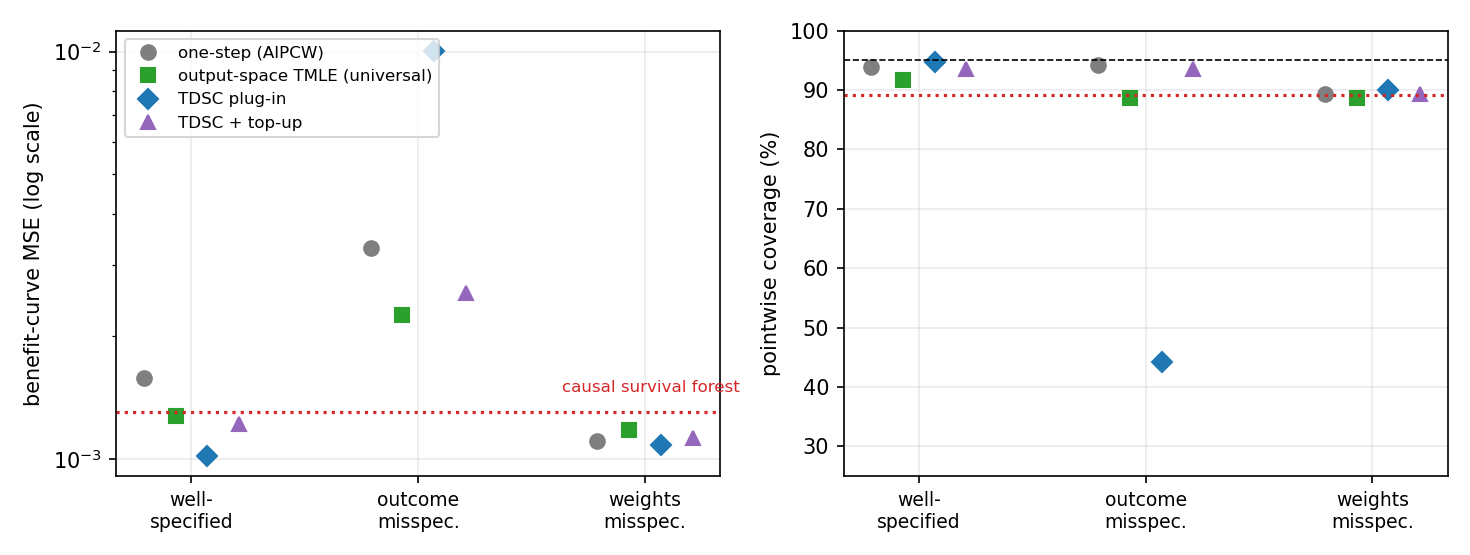
\includegraphics[width=0.95\linewidth]{../figures/comparators.png}
\caption{Head-to-head comparison across nuisance scenarios (benefit-curve MSE, log scale; pointwise coverage, 95\% dashed). The three same-nuisance estimators order one-step $\to$ output-space TMLE $\to$ TDSC when well-specified; under outcome misspecification the weight-space update is the most exposed while the one-step alone stays nominal. The causal survival forest (own nuisances, horizons 5--25) appears as the dotted reference.}
\label{fig:comp}
\end{figure}

\begin{table}[t]
\centering
\caption{Sample-size scaling, benefit curve (well-specified, Table~\ref{tab:main} configuration; 150/200/150 replications).}
\label{tab:nscale}
\begin{tabular}{rlccccc}
\toprule
$n$ & Estimator & Bias & $n\times$MSE & Coverage & CI width & Simult.\ band \\
\midrule
 500 & one-step & 0.0056 & 2.10 & 94.8\% & 0.232 & --- \\
     & TDSC     & 0.0140 & 2.77 & 91.4\% & 0.198 & 85.3\% \\
\midrule
1000 & one-step & 0.0057 & 1.73 & 95.1\% & 0.151 & --- \\
     & TDSC     & 0.0021 & 1.49 & 95.6\% & 0.140 & 94.0\% \\
\midrule
2000 & one-step & 0.0025 & 1.43 & 93.7\% & 0.096 & --- \\
     & TDSC     & 0.0014 & 1.02 & 96.2\% & 0.093 & 96.7\% \\
\bottomrule
\end{tabular}
\end{table}

\begin{table}[t]
\centering
\caption{Nuisance-misspecification grid, benefit curve ($n=1000$, $K=30$, 150 replications per arm; coverage MC SE $\approx$ 1.8pp). \emph{outcome mis.}: outcome hazards blinded to $x_1, x_3$; \emph{weights mis.}: propensity and censoring models blinded to $x_1, x_2$. Propensity is fit by a standalone network (not Table~\ref{tab:main}'s trunk head), so well-specified cells are not directly comparable to Table~\ref{tab:main}. The isotonized row changes only the point estimate; the safeguard row changes only the interval (its nonparametric SE equals the one-step's, hence the equal widths).}
\label{tab:mis}
\begin{tabular}{llcccc}
\toprule
Scenario & Estimator & Bias & MSE & Coverage & CI width \\
\midrule
well-specified & one-step            & 0.0051 & 0.00155 & 94.5\% & 0.144 \\
               & one-step, isotonized& 0.0051 & 0.00154 & ---    & ---   \\
               & TDSC                & \textbf{0.0036} & \textbf{0.00103} & 95.7\% & \textbf{0.135} \\
\midrule
outcome mis.   & naive plug-in       & 0.1922 & 0.04110 & ---    & ---   \\
               & one-step            & 0.0135 & \textbf{0.00345} & \textbf{95.0\%} & 0.197 \\
               & TDSC                & 0.0119 & 0.01860 & 64.6\% & 0.156 \\
               & TDSC + top-up       & 0.0265 & 0.01325 & 84.3\% & 0.156 \\
               & \ \ + nonpar.\ SE (safeguard) & --- & --- & 88.8\% & 0.197 \\
\midrule
weights mis.   & IPTW$\times$IPCW KM & 0.0760 & 0.00720 & ---    & ---   \\
               & one-step            & 0.0114 & 0.00111 & 89.4\% & 0.111 \\
               & TDSC                & 0.0111 & 0.00114 & 89.2\% & 0.111 \\
\bottomrule
\end{tabular}
\end{table}

\begin{table}[t]
\centering
\caption{Benefit curve $S_1(t)-S_0(t)$, time-averaged over 30 points ($n=1000$, $K=30$; 200 replications, coverage MC SE $\approx$ 1.5pp). Bias is the time-averaged absolute Monte Carlo bias. The paired TDSC$-$one-step MSE difference is $-0.00024$ (MC SE $0.00026$).}
\label{tab:main}
\begin{tabular}{lcccc}
\toprule
 & Bias & MSE & Coverage (ptwise) & CI width \\
\midrule
Naive neural plug-in & 0.0213 & 0.0026 & --- & --- \\
Unadjusted KM        & 0.1212 & 0.0163 & --- & --- \\
One-step (AIPCW)     & 0.0057 & 0.0017 & 95.1\% & 0.151 \\
TDSC (ours)          & \textbf{0.0021} & \textbf{0.0015} & 95.6\% & \textbf{0.140} \\
\midrule
$\Delta_{\mathrm{RMST}}$: one-step & bias $-$0.161 & MSE \textbf{0.53} & 96.5\% & 2.87 \\
$\Delta_{\mathrm{RMST}}$: TDSC     & bias \textbf{0.007} & MSE 0.79 & 95.5\% & 2.69 \\
\midrule
TDSC simultaneous band & \multicolumn{2}{c}{coverage 94.0\% (whole curve)} & \multicolumn{2}{c}{band width 0.207} \\
\bottomrule
\end{tabular}
\end{table}

\begin{figure}[t]
\centering
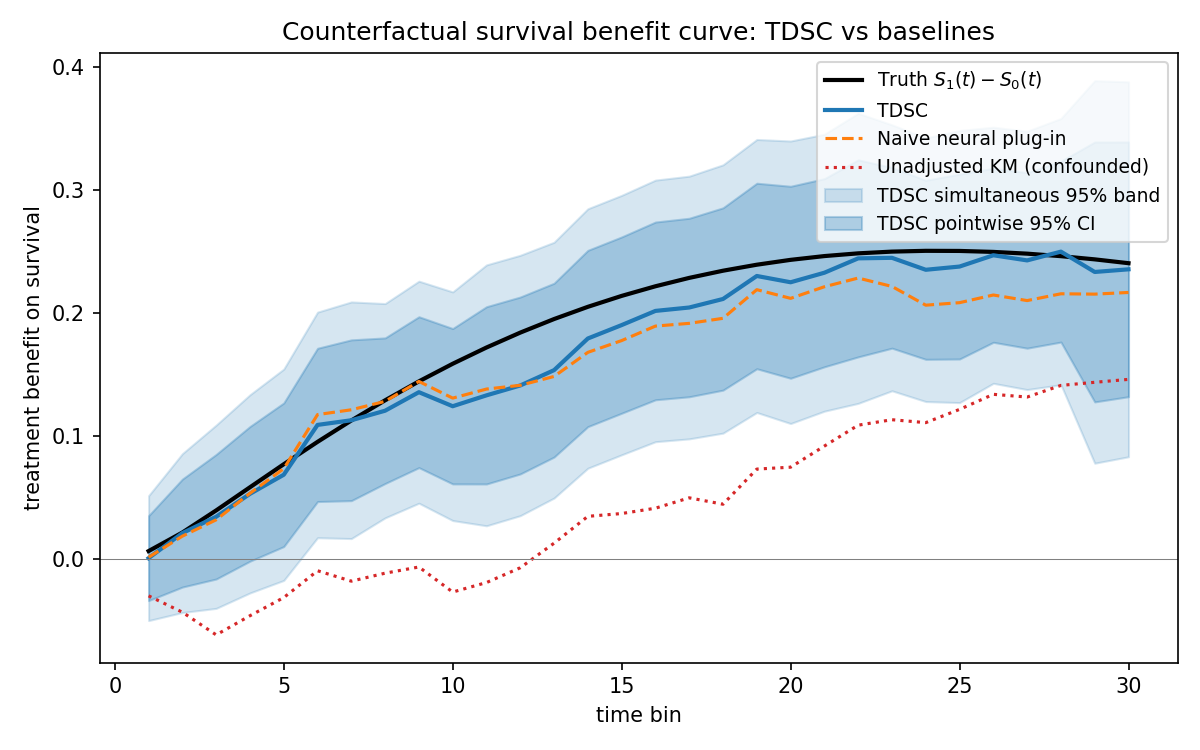
\includegraphics[width=0.8\linewidth]{../figures/benefit_curve.png}
\caption{One replication ($n=1000$, seed 7). The TDSC benefit curve tracks the truth, which lies inside both the pointwise CI and the simultaneous band; the naive plug-in drifts low at later times, and unadjusted KM is severely biased (wrong-signed at early times).}
\label{fig:money}
\end{figure}

\section{Discussion}\label{sec:disc}

TDSC turns a two-headed neural survival network into a valid estimator of population treatment benefit at the cost of a few ridge regressions after training, and the misspecification grid gives the method an honest operating envelope: prefer TDSC when the initial network fits well (narrower intervals at nominal coverage, gains not attributable to monotonicity; $n\gtrsim 1000$ in our design), and fall back when diagnostics (large full-EIF residual means---the top-up magnitudes---or a large projection residual) suggest otherwise or the sample is small---the safeguarded top-up repairs most of the coverage loss, but under gross outcome misspecification, and at $n=500$, only the one-step is fully reliable. The remaining work: (i) the cross-fitted variant under misspecification and at small $n$---it is nominal and modestly less efficient in the well-specified case (Section~\ref{sec:sims}), and the settings where no-split inference failed are exactly where its guarantee should earn its keep; (ii) sensitivity to the ridge penalty, targeting-layer choice, and weight-truncation levels (Appendix~\ref{app:repro}); (iii) \emph{calibration-for-benefit}---targeting arm-specific curves within strata of the network's own predicted benefit, the estimand used to validate individualized-benefit models against randomized trials---and application on frozen pretrained encoders (e.g.\ pathology foundation models), which the last-layer construction supports directly.

\appendix
\section{Reproducibility}\label{app:repro}
All code, raw Monte Carlo stores, and the exact scripts behind every table are at \url{https://github.com/blind-contours/tdsc}. Networks: trunk $d\to64\to64$ (ELU); propensity head $64\to64\to1$; per-arm outcome heads $64\to64\to K$; censoring network $(d{+}1)\to64\to64\to(K{-}1)$. Training: full-batch Adam, lr $10^{-3}$, max 500 epochs, early stopping (patience 25) on a 20\% validation split, propensity loss weight 1.0. Targeting: ridge scale $\lambda = 0.01\times\mathrm{mean\,diag}(G^\top G)$ (a finite-sample stabilizer; the theory requires only that the relative ridge vanish, Section~\ref{sec:theory}); $\gamma_0=1$ with up to 12 halvings; max 50 iterations; stopping tolerance $\widehat{\mathrm{sd}}(D^{w}_j)/(\sqrt n \log n)$ on the projected means. Truncation: $\hat g\in[0.05,0.95]$, $\hat S_c \ge 0.05$, conditional survival floored at $10^{-3}$ inside \eqref{eq:eif}. Bands: 1000 Gaussian-multiplier draws. Cross-fitting: $V=5$, fold networks trained and targeted on complements with the same hyperparameters. Output-space TMLE: per-coordinate logistic fluctuations solved by Newton steps ($\epsilon$ clipped to $[-5,5]$), recomputing the clever covariate each round, up to 25 rounds per coordinate, same $\mathrm{sd}/(\sqrt n\log n)$ tolerance. Causal survival forests: \texttt{grf} 2.6.1, \texttt{causal\_survival\_forest} with \texttt{target = "survival.probability"}, 1{,}000 trees, default tuning, one forest per horizon $\{5,10,15,20,25\}$, population effect and SE from \texttt{average\_treatment\_effect}. The main tables use the no-split estimator (Table~\ref{tab:main} with the trunk propensity head; Tables~\ref{tab:mis} and~\ref{tab:comp} with a standalone propensity network). Truth: Monte Carlo integration over $4\times10^5$ covariate draws.

\section{Proof sketches}\label{app:proofs}

\paragraph{Theorem~\ref{thm:main}.} All influence functions in this proof are the nonparametric EIFs \eqref{eq:eif}; superscripts are omitted. Per coordinate, since $\widehat\Psi^{+}_j = \Psi_j(\hat P) + \Pn\widehat D_j$ and the EIF has the form $\widehat D_j = \widehat D_j^{\mathrm{mart}} + \hat S_j - \Psi_j(\hat P)$, the standard one-step decomposition holds exactly:
\[
\widehat\Psi^{+}_j - \Psi_j(P_0) \;=\; \Pn D_{0,j} \;+\; (\Pn - P_0)\big(\widehat D_j - D_{0,j}\big) \;+\; R_{2,j},
\qquad R_{2,j} = P_0 \widehat D_j + \Psi_j(\hat P) - \Psi_j(P_0).
\]
For the remainder, the survival EIF is exact to second order: writing $S_{h}(k)=\prod_{j\le k}(1-h(j))$ for the conditional survival under a hazard $h$, the telescoping identity
$S_{\hat h}(t) - S_{h_0}(t) = \sum_{k\le t} S_{h_0}(k-1)\,\big(h_0(k)-\hat h(k)\big)\,S_{\hat h}(t)/S_{\hat h}(k)$
gives $R_{2,j}$ as a sum over $k\le t$ of integrals of $\{\hat h(k) - h_0(k)\}$ against $\{\hat g\hat S_c(k-1) - g_0 S_{c,0}(k-1)\}/\{\hat g \hat S_c(k-1)\}$-type differences; under the positivity bounds of Assumption~\ref{a:id}, Cauchy--Schwarz gives $|R_{2,j}| \lesssim \|\hat h - h_0\|_{P_0}(\|\hat g - g_0\|_{P_0} + \|\hat S_c - S_{c,0}\|_{P_0}) = o_p(n^{-1/2})$ by Assumption~\ref{a:rates}, applied to the targeted per-fold hazards (this display also proves Proposition~\ref{prop:dr}: $R_2$ vanishes if either factor's limit is correct). For the empirical-process term, cross-fitting makes $\widehat D_j$ independent of the fold on which $(\Pn-P_0)$ is evaluated, so conditional on the training folds, $(\Pn - P_0)(\widehat D_j - D_{0,j}) = o_p(n^{-1/2})$ whenever $\|\widehat D_j - D_{0,j}\|_{P_0} = o_p(1)$, which follows from the individual nuisance consistency in Assumption~\ref{a:rates} (targeting, which moves $\vartheta$ along the score span, is designed to improve rather than degrade those rates). Summing folds yields the coordinate-wise expansion; joint convergence follows from the multivariate CLT applied to the stacked $D_0$. Proposition~\ref{prop:plugin} is \citet[Thms.~3.1--3.2]{li2025tda} applied verbatim to the cross-fitted plug-in, with superefficiency from their Theorem~3.2 under (C1)--(C2).

\paragraph{Corollary~\ref{cor:contrasts} and Proposition~\ref{prop:band}.} Both maps are bounded linear in $\Psi$, so asymptotic linearity transfers with the transformed influence functions. Given joint normality with consistently estimated $\Sigma_0$ (IF second moments), the conditional multiplier process $n^{-1/2}\sum_i \xi_i \widehat D_{\beta,t}(O_i)$ converges weakly to the same Gaussian limit (conditional multiplier CLT), so its sup-quantile is consistent for the sup-quantile of the limit; the $c^*\ge1.96$ floor only enlarges the band.

\paragraph{Proposition~\ref{prop:dr}.} By definition $\widehat\Psi^{+}_j = \Pn[\hat S(t\mid a, X)] + \Pn \widehat D_j$, which is precisely the AIPCW one-step at nuisances $(\hat h^{\mathrm{targ}}, \hat g, \hat S_c)$. Its population bias is the $R_2$ term above evaluated at those limits, which vanishes under either-arm consistency. \hfill$\square$

\bibliographystyle{plainnat}
\begin{thebibliography}{12}

\bibitem[Cai and van~der Laan(2020)]{cai2020}
W.~Cai and M.~J. van~der Laan.
\newblock One-step targeted maximum likelihood estimation for time-to-event outcomes.
\newblock \emph{Biometrics}, 76(3):722--733, 2020.
\newblock \url{https://doi.org/10.1111/biom.13172}.

\bibitem[Chapfuwa et~al.(2021)]{chapfuwa2021}
P.~Chapfuwa, S.~Assaad, S.~Zeng, M.~J. Pencina, L.~Carin, and R.~Henao.
\newblock Enabling counterfactual survival analysis with balanced representations.
\newblock In \emph{Proceedings of the Conference on Health, Inference, and Learning (CHIL)}, 2021.
\newblock \url{https://doi.org/10.1145/3450439.3451875}.

\bibitem[Chernozhukov et~al.(2018)]{chernozhukov2018dml}
V.~Chernozhukov, D.~Chetverikov, M.~Demirer, E.~Duflo, C.~Hansen, W.~Newey, and J.~Robins.
\newblock Double/debiased machine learning for treatment and structural parameters.
\newblock \emph{The Econometrics Journal}, 21(1):C1--C68, 2018.
\newblock \url{https://doi.org/10.1111/ectj.12097}.

\bibitem[Cui et~al.(2023)]{cui2023csf}
Y.~Cui, M.~R. Kosorok, E.~Sverdrup, S.~Wager, and R.~Zhu.
\newblock Estimating heterogeneous treatment effects with right-censored data via causal survival forests.
\newblock \emph{Journal of the Royal Statistical Society: Series B}, 85(2):179--211, 2023.
\newblock \url{https://doi.org/10.1093/jrsssb/qkac001}.

\bibitem[Curth et~al.(2021)]{curth2021survite}
A.~Curth, C.~Lee, and M.~van~der Schaar.
\newblock SurvITE: Learning heterogeneous treatment effects from time-to-event data.
\newblock \emph{Advances in Neural Information Processing Systems}, 34, 2021.
\newblock \url{https://proceedings.neurips.cc/paper/2021/hash/e0eacd983971634327ae1819ea8b6214-Abstract.html}.

\bibitem[Kennedy(2024)]{kennedy2024review}
E.~H. Kennedy.
\newblock Semiparametric doubly robust targeted double machine learning: a review.
\newblock In \emph{Handbook of Statistical Methods for Precision Medicine}. Chapman \& Hall/CRC, 2024.
\newblock \url{https://arxiv.org/abs/2203.06469}.

\bibitem[Li et~al.(2025)]{li2025tda}
Y.~Li, D.~McCoy, N.~Gunter, K.~Lee, A.~Schuler, and M.~J. van~der Laan.
\newblock Targeted deep architectures: A TMLE-based framework for robust causal inference in neural networks.
\newblock \emph{arXiv preprint arXiv:2507.12435}, 2025.
\newblock \url{https://arxiv.org/abs/2507.12435}.

\bibitem[Moore and van~der Laan(2009)]{moore2009}
K.~L. Moore and M.~J. van~der Laan.
\newblock Increasing power in randomized trials with right censored outcomes through covariate adjustment.
\newblock \emph{Journal of Biopharmaceutical Statistics}, 19(6):1099--1131, 2009.
\newblock \url{https://doi.org/10.1080/10543400903243017}.

\bibitem[Rytgaard and van~der Laan(2024)]{rytgaard2024}
H.~C.~W. Rytgaard and M.~J. van~der Laan.
\newblock One-step targeted maximum likelihood estimation for targeting cause-specific absolute risks and survival curves.
\newblock \emph{Biometrika}, 111(1):129--145, 2024.
\newblock \url{https://doi.org/10.1093/biomet/asad033}.

\bibitem[Shi et~al.(2019)]{shi2019dragonnet}
C.~Shi, D.~Blei, and V.~Veitch.
\newblock Adapting neural networks for the estimation of treatment effects.
\newblock \emph{Advances in Neural Information Processing Systems}, 32, 2019.
\newblock \url{https://proceedings.neurips.cc/paper/2019/hash/8fb5f8be2aa9d6c64a04e3ab9f63feee-Abstract.html}.

\bibitem[Zheng and van~der Laan(2011)]{zheng2011cvtmle}
W.~Zheng and M.~J. van~der Laan.
\newblock Cross-validated targeted minimum-loss-based estimation.
\newblock In \emph{Targeted Learning: Causal Inference for Observational and Experimental Data}, pages 459--474. Springer, 2011.
\newblock \url{https://doi.org/10.1007/978-1-4419-9782-1_27}.

\bibitem[van~der Laan and Rose(2011)]{vdl2011tl}
M.~J. van~der Laan and S.~Rose.
\newblock \emph{Targeted Learning: Causal Inference for Observational and Experimental Data}.
\newblock Springer, 2011.
\newblock \url{https://doi.org/10.1007/978-1-4419-9782-1}.

\bibitem[van~der Laan et~al.(2023)]{vdl2023adml}
L.~van~der Laan, M.~Carone, A.~Luedtke, and M.~J. van~der Laan.
\newblock Adaptive debiased machine learning using data-driven model selection techniques.
\newblock \emph{arXiv preprint arXiv:2307.12544}, 2023.
\newblock \url{https://arxiv.org/abs/2307.12544}.

\end{thebibliography}

\end{document}
